\chapter{Estratégia de preparação para o TCE-MA}

\section{Leitura estratégica do edital}

\begin{teoria}[peso das provas]
A objetiva é composta por 40 questões de conhecimentos gerais e 60 de conhecimentos específicos. As gerais valem 1 ponto cada e as específicas valem 2 pontos cada. Assim, a objetiva soma 160 pontos: \textbf{25\%} da pontuação está nos conhecimentos gerais e \textbf{75\%} nos específicos.

Isso não significa abandonar conhecimentos gerais. Significa estudar de forma proporcional ao retorno: português, legislação, controle externo e direitos costumam decidir classificação quando os candidatos tecnicamente fortes ficam próximos nos específicos.
\end{teoria}

\begin{center}
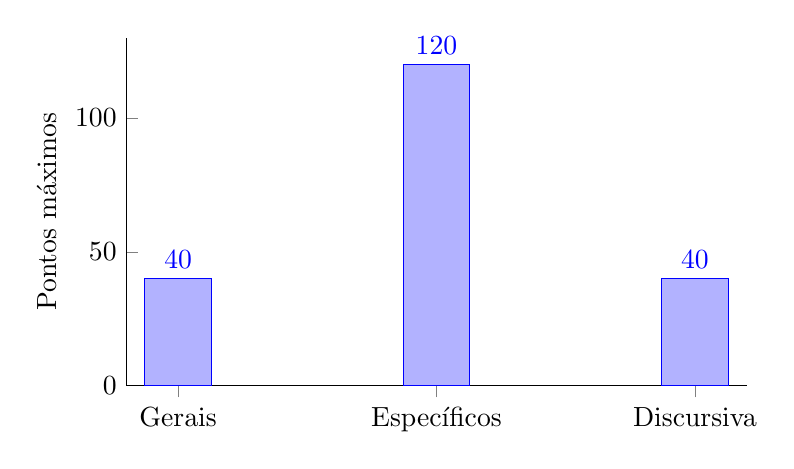
\begin{tikzpicture}
\begin{axis}[
 ybar,bar width=24pt,
 width=.78\textwidth,height=6cm,
 ylabel={Pontos máximos},
 symbolic x coords={Gerais,Específicos,Discursiva},xtick=data,
 ymin=0,ymax=130,
 nodes near coords,
 axis lines*=left]
\addplot coordinates {(Gerais,40) (Específicos,120) (Discursiva,40)};
\end{axis}
\end{tikzpicture}
\end{center}

\section{O que muda por ser Auditor de TI}

O edital não cobra apenas administração de tecnologia. A função mistura \termo{profundidade técnica}, \termo{governança}, \termo{contratação pública}, \termo{dados} e \termo{auditoria}. Em uma questão avançada, a banca pode combinar, por exemplo, evidência de auditoria, logs em nuvem, segregação de funções, IAM e LGPD.

\begin{cebraspe}
Ao estudar um conceito técnico, responda sempre quatro perguntas:
\begin{enumerate}
\item O que é e qual problema resolve?
\item Qual é a diferença para conceitos próximos?
\item Que risco surge quando é mal implementado?
\item Como um auditor obteria evidência de que o controle funciona?
\end{enumerate}
Essa quarta pergunta converte conhecimento de TI em conhecimento de Auditor/TI.
\end{cebraspe}

\section{Ciclo de estudo recomendado}

Com 107 dias entre 14/08/2026 e 29/11/2026, a preparação pode ser dividida em quatro ciclos.

\begin{table}[ht]
\centering
\begin{tabularx}{\textwidth}{>{\bfseries}l l X}
\toprule
Fase & Janela & Objetivo \\
\midrule
1. Cobertura & agosto--setembro & Fechar todo o edital, priorizando específicos. \\
2. Consolidação & outubro & Revisões, questões N2--N4 e discursivas. \\
3. Prova & início de novembro & Simulados completos, correção de lacunas e revisão normativa. \\
4. Reta final & últimas 2 semanas & Revisão de mapas, erros recorrentes, legislação seca e peças técnicas. \\
\bottomrule
\end{tabularx}
\end{table}

\section{Matriz de prioridade}

\begin{table}[ht]
\centering
\small
\begin{tabularx}{\textwidth}{l c X}
\toprule
Bloco & Prioridade & Razão \\
\midrule
Infraestrutura + Segurança + Nuvem & Muito alta & Grande extensão, integração natural e forte potencial de casos. \\
Dados + IA & Muito alta & Conteúdo moderno, técnico e aderente às atribuições do cargo. \\
Governança + Contratações & Muito alta & Diferencial de auditor público de TI. \\
Engenharia de Software & Alta & DevOps, testes, CI/CD, Kubernetes e requisitos são cobrados de forma integrada. \\
Auditoria do setor público & Muito alta & Está no específico e sustenta a discursiva. \\
Controle Externo + Legislação TCE & Alta & Contextualizam a atuação institucional. \\
Português + Raciocínio Lógico & Média/alta & Elevado potencial de ganho por treino. \\
História/Geografia + Direitos Humanos & Média & Conteúdo objetivo e revisável por mapas e questões. \\
\bottomrule
\end{tabularx}
\end{table}

\section{Como usar N1--N4}

\begin{itemize}
\item \nivel{N1} identificar definições, propriedades e componentes.
\item \nivel{N2} aplicar conceitos em um cenário simples.
\item \nivel{N3} resolver questão com integração de dois ou mais tópicos, distratores plausíveis e detalhes normativos.
\item \nivel{N4} enfrentar estudo de caso típico de Auditor/TI, justificando decisão, risco, evidência e recomendação.
\end{itemize}

\section{Caderno de erros}

Para cada erro, registre: assunto, causa, regra correta, motivo do distrator ter parecido correto e uma frase de recuperação. Classifique a causa em: \emph{desconhecimento}, \emph{confusão conceitual}, \emph{leitura}, \emph{cálculo}, \emph{memória normativa} ou \emph{gestão de tempo}. A revisão deve atacar a causa, não apenas repetir a questão.

\begin{resumo}
\textbf{Regra central:} específicos carregam 75\% da objetiva, mas a aprovação exige equilíbrio. Estude TI como auditor: conceito + risco + controle + evidência. Resolva N1 para fundação, N2 para aplicação, N3 para prova e N4 para diferenciação.
\end{resumo}
